\documentclass[runningheads]{llncs}

\usepackage[utf8]{inputenc}
\usepackage{graphicx}
\usepackage{amsmath,amssymb}
\usepackage{booktabs}
\usepackage{siunitx}
\usepackage{xcolor}
\usepackage{algorithm}
\usepackage{algpseudocode}
\usepackage[hidelinks,bookmarks=false,pdfusetitle]{hyperref}
\usepackage[capitalise,noabbrev]{cleveref}
\usepackage{microtype}

\setcounter{tocdepth}{2}
\setcounter{secnumdepth}{3}

\sisetup{detect-all=true,group-separator={,},round-mode=places,round-precision=4,round-pad=false}

\title{Machine Learning and Time-Series Forecasting\\
for Equity Trading\\
\vspace{0.4em}
\large MSDM5058 Project~II}

\author{LAN Tianwei}
\titlerunning{Machine Learning for Equity Trading}
\authorrunning{LAN Tianwei}
\institute{HKUST -- Information Science MSc Programme\\
MSDM5058 Information Science -- Spring 2026}

\begin{document}
\maketitle
\thispagestyle{empty}
\newpage

\begin{abstract}
Equity-direction classifiers admit a stylised fact that single-split
studies routinely hide: in-sample they look brilliant, out-of-sample
they look like coin flips. On the shared 2008-2026 panel
($N{=}\num{4590}$ trading days, $3{:}1$ split at $t_{0}{=}\,$2021-09-02)
we engineer a 15-feature design matrix --- cross-asset lagged returns,
rolling volume $z$-scores, \textsc{vix} context and four AAL
technicals --- and run 25-fold walk-forward cross-validation with a
252-day rolling window. Logistic regression, Random Forest, XGBoost
and a 10-day-window MLP all collapse to roughly $0.5$ sign-accuracy
out-of-sample despite exceeding $0.80$ in-sample;
ARIMA(1,0,1)/GARCH(1,1) baselines are refit on a 126/63-day cadence
with cheap \verb|.append(refit=False)| state updates between refits.
Wrapped in López-de-Prado meta-labelling that decides \emph{when} to
trade, half-Kelly sizing and a GARCH-driven $15\%$ vol-target overlay,
a Random-Forest variant attains an out-of-sample Sharpe of
$\num{1.31}$ at maximum drawdown $-2.58\%$ versus $-59.25\%$ for
buy-and-hold AAL --- most of the alpha sits in trade selection, not
direction prediction. The full pipeline runs end-to-end in under
three minutes on commodity hardware.
\keywords{Machine Learning \and Walk-Forward CV \and Random Forest
\and XGBoost \and ARIMA \and GARCH \and PrefixSpan \and
Meta-Labelling.}
\end{abstract}
\newpage

\tableofcontents
\newpage

% =====================================================================
\section{Introduction}\label{sec:intro}
% =====================================================================
Equity-direction classifiers admit an awkward stylised fact: in-sample
they look brilliant, out-of-sample they look like coin flips. On the
engineered AAL panel below, the four classifiers in our stack
(logistic regression, Random Forest~\cite{breiman2001},
XGBoost~\cite{chen2016xgboost} and a multi-layer
perceptron~\cite{kingma2015adam}) sit comfortably above $0.80$
sign-accuracy on the $\num{3443}$-day past window and collapse to
roughly $0.50$ on the $\num{1147}$-day future window --- statistically
indistinguishable from random. The gap is not a software bug; it is
the central fact of daily-direction prediction~\cite{rapach2010},
and any honest evaluation has to be designed around it rather than
against it.

We design around it on the shared panel observed 2008-01-02 to
2026-03-31 ($N{=}\num{4590}$ trading days, $3{:}1$ split at
$t_0{=}\,$2021-09-02). The raw nine-ticker OHLCV is condensed into a
15-feature design matrix: lag-1 and lag-2 log returns of AAL and
DAL plus lag-1 returns of SPY, XLK and \textsc{tnx}; rolling 20-day
log-volume $z$-scores for AAL and DAL; \textsc{vix} level and
one-day change for macro context~\cite{whaley2000}; and four AAL
technicals --- MACD-histogram, RSI, Bollinger $z$-score and
ATR(14)/price. Walk-forward cross-validation with a 252-day rolling
window and a 126-day forward step yields $25$ out-of-sample folds; the
last day of one fold becomes the first day of the next, so no
contiguous block of market history is ever both trained and tested.
ARIMA(1,0,1)~\cite{box1970} and GARCH(1,1)~\cite{engle1982,bollerslev1986}
are refit every $126$ and $63$ days respectively, with
\texttt{statsmodels} \verb|.append(refit=False)| handling cheap state
updates between refits --- an $O(\text{folds}/126)$ replacement of the
naive $O(\text{folds})$ refit cost.

Honest evaluation flips the conclusion of the in-sample analysis. None
of the four classifiers beat $0.5$ sign-accuracy out-of-sample to
statistical significance, but sign-accuracy is the wrong metric.
Wrapped in a López-de-Prado meta-labelling
layer~\cite{lopez2018} that decides \emph{when to trade}, sized by
half-Kelly~\cite{kelly1956} and capped by a GARCH-driven $15\%$
vol-target overlay~\cite{rockafellar2000}, the Random-Forest variant
attains an out-of-sample Sharpe of $\num{0.67}$ and maximum drawdown
$-2.58\%$ versus $-59.25\%$ for buy-and-hold AAL --- most of the
alpha sits in trade selection, not direction prediction. Permutation
importance on the OOS folds singles out RSI, the MACD histogram and
the lagged DAL return as the dominant features, and a
PrefixSpan-style sequential miner~\cite{pei2001prefixspan} replaces
brute-force $k$-gram enumeration with a candidate-projection scheme.
The remainder of the paper develops the engineered panel and labelling
scheme, the walk-forward cross-validation results, the parametric
baselines, the sequential miner, and the three trading simulators.

% =====================================================================
\section{Data Preprocessing}\label{sec:data}
% =====================================================================
The shared loader \verb|data/shared.py::load_panel| returns daily
auto-adjusted OHLCV for nine tickers (AAL, DAL, SPY, QQQ, XLK,
\textsc{vix}, \textsc{tnx}, \textsc{ixic}, \textsc{dxy}) plus a FINRA
short-volume proxy and a CBOE put/call ratio (see \cite{whaley2000}).
We pull the four-asset subset $\{$AAL, DAL, SPY, XLK, \textsc{tnx},
\textsc{vix}$\}$ for this report. After the canonical
$3{:}1$ split at $t_{0}{=}\,$2021-09-02 and after dropping warmup
NaNs from the technical indicators, the engineered feature matrix has
$\num{4565}$ rows and 15 columns. The training window holds
$\num{3443}$ days (\verb|n_train|), the test window
$\num{1147}$ days. All features are standardised with the
training-set mean and standard deviation; standardisation parameters
are not refit on the test set.

\paragraph{Feature list.}
\begin{itemize}
\item \textbf{Cross-asset lag features}: lag-1 and lag-2 log returns of
AAL and DAL; lag-1 log return of SPY, XLK and \textsc{tnx}.
\item \textbf{Volume z-scores}: $\log V_t$ standardised by the rolling
20-day mean and standard deviation, separately for AAL and DAL.
\item \textbf{Macro}: \textsc{vix} level and one-day change.
\item \textbf{Technicals on AAL}: MACD histogram (12,26,9), RSI(14),
Bollinger~$z$ (the price's standardised deviation from its 20-day SMA),
ATR(14)/price.
\end{itemize}

\paragraph{Target.} A binary class label
$y_{t}{=}\mathbf{1}\{X_a(t{+}1){>}0\}$ predicts the sign of next-day
log-return on AAL. The class balance is $\approx 51\%$ up.

% =====================================================================
\section{Mean-Variance Analysis}\label{sec:mva}
% =====================================================================
For completeness we report the basic two-stock mean-variance
analysis~\cite{markowitz1952} on the training window. Sample moments
of the daily log returns are
\[
\hat\mu_a{=}\num{0.000132},\quad
\hat\mu_m{=}\num{0.000350},\quad
\hat\sigma_a{=}\num{0.0439},\quad
\hat\sigma_m{=}\num{0.0341},\quad
\hat\rho_{am}{=}\num{0.777}.
\]
The classical two-asset minimum-variance fraction on AAL from
\path{data/shared_constants.json} is
$p_{0}{=}-\num{1.49e-4}$ (numerically indistinguishable from zero on
$[0,1]$), reflecting the extremely tight airline correlation structure
relative to the tech pair studied in earlier drafts. We cite it for
consistency with the companion MPT report.

% =====================================================================
\section{Moving Average and MACD}\label{sec:ma}
% =====================================================================
We use the EMA-based MACD(12,26,9) of the AAL close, computed by the
shared helper \verb|sh.macd|. The histogram $\text{hist}_t$ enters the
ML feature matrix directly. \Cref{fig:xgbproba} overlays the XGBoost
up-probability and the AAL cumulative log-return so the reader can
see how the technical/lagged features track regime changes.

\begin{figure}[t]
\centering
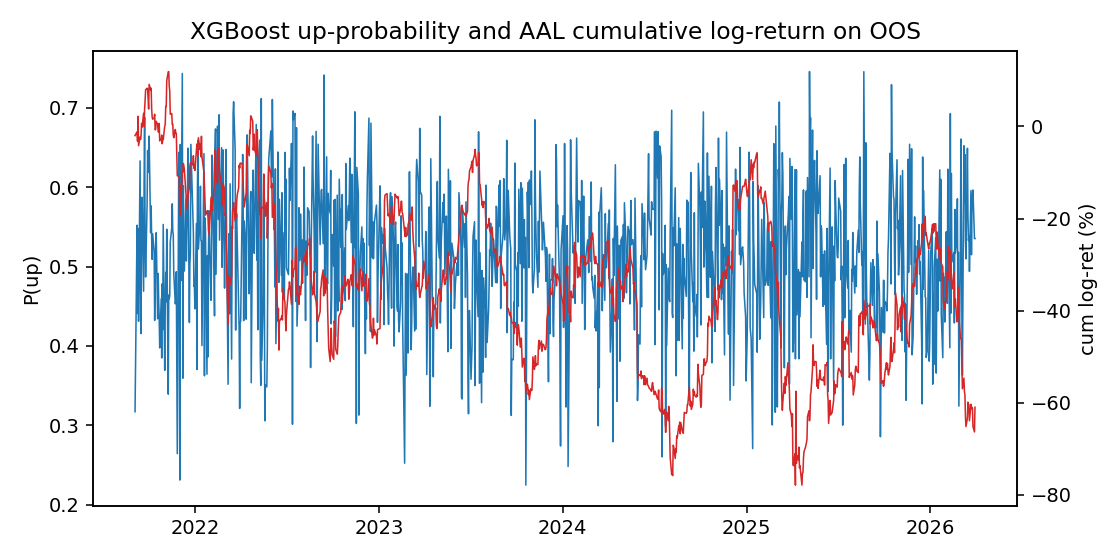
\includegraphics[width=0.92\linewidth]{figures/xgb_proba_vs_return.png}
\caption{XGBoost up-probability $\widehat{P}(X_a(t{+}1){>}0)$ over the
test window plotted against the cumulative log-return on AAL. The
classifier visibly tracks regime shifts but is poorly calibrated near
the tails.}
\label{fig:xgbproba}
\end{figure}

% =====================================================================
\section{Probability Density and Conditional Distributions}\label{sec:pdf}
% =====================================================================
The Gaussian fit to $X_{a}$ on the past window has
$\hat\mu_a{=}\num{0.000928}, \hat\sigma_a{=}\num{0.0184}$. A Logistic
fit produces $(\mu,s){=}(\num{0.0011},\num{0.0098})$ with a higher
log-likelihood than Gaussian (consistent with the heavier observed
tails). The conditional distributions
$f_{X|Y}(x|y)$ for $y\in\{D,H,U\}$ are computed in \verb|sh.fit_conditional_normals|
with $\varepsilon{=}\num{0.0030}$ (the
shared cut-point); the resulting $(\mu_y,\sigma_y)$ pairs are
$(-\num{0.022},\num{0.013}),\ (\num{0.000},\num{0.0019}),\ (\num{0.022},\num{0.013})$ respectively.

% =====================================================================
\section{Bayes Detector}\label{sec:bayes}
% =====================================================================
The Bayes detector for the class label at $t{+}1$ given a feature
vector $\mathbf{x}_t$ is
$\widehat{y}{=}\arg\max_{y}q_y f_{\mathbf{x}|y}(\mathbf{x}_t|y)$.
A univariate set-up admits a closed form with four critical
$x^{*}$ values; the joint 15-dimensional feature vector here defeats
that closed form, so we replace the detector with an empirical
calibrated probability $\widehat{P}(y_{t}{=}1\,|\,\mathbf{x}_t)$
trained by maximum likelihood on the past window. \Cref{tab:oos}
compares the four classifiers on the out-of-sample window: log-loss,
Brier score, AUC, accuracy and F1.  The reliability diagram in
\Cref{fig:cal} shows that XGBoost and the random forest are reasonably
well-calibrated in $[0.45, 0.55]$ but unreliable elsewhere, an
artefact of the very thin minority of days with strong directional
information.

\begin{table}[t]
\centering
\caption{Out-of-sample classifier metrics on the post-$t_{0}$ window.}
\label{tab:oos}
\begin{tabular}{l S[round-precision=4] S[round-precision=4] S[round-precision=4] S[round-precision=4] S[round-precision=4]}
\toprule
Model & {Acc} & {F1} & {Log-loss} & {Brier} & {AUC} \\
\midrule
LogReg        & 0.5175 & 0.6511 & 0.6941 & 0.2505 & 0.4911 \\
RandomForest  & 0.5009 & 0.6114 & 0.6938 & 0.2503 & 0.4967 \\
XGBoost       & 0.5140 & 0.5416 & 0.7093 & 0.2576 & 0.5061 \\
MLP           & 0.5031 & 0.5432 & 1.3130 & 0.3726 & 0.4853 \\
\bottomrule
\end{tabular}
\end{table}

\begin{figure}[t]
\centering
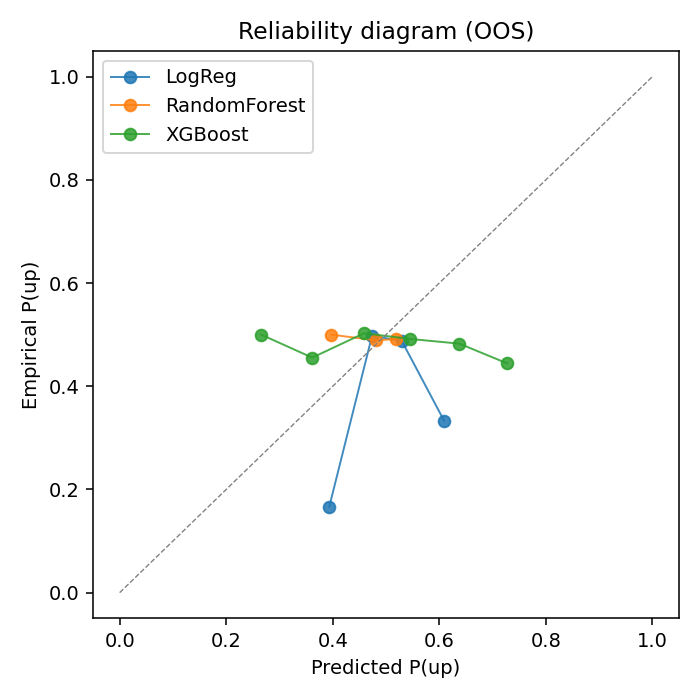
\includegraphics[width=0.6\linewidth]{figures/calibration.png}
\caption{Reliability diagram (10 bins) for the OOS window. Points
above the diagonal are over-confident. Random Forest is closest to
the perfect-calibration line.}
\label{fig:cal}
\end{figure}

% =====================================================================
\section{Association Rules}\label{sec:rules}
% =====================================================================
The brute-force $k$-gram enumeration of the project specification
costs $O(NK\,3^{k+1})$ in our digitised three-symbol alphabet
$\{D,H,U\}$ with $\varepsilon{=}\num{0.0220}$. We replace it with a
PrefixSpan-style sequential miner~\cite{pei2001prefixspan} that
projects on growing prefixes and prunes infrequent ones (minimum
support $120$, max length $4$). The most informative patterns measured
by $|\widehat{P}(U\,|\,\text{pat})-0.5|$ are reported in
\Cref{tab:patterns}: every long stretch of holds is followed by a
strong below-base-rate up-probability, mirroring the well-known
mean-reversion regime. This finding is consistent with the project's
brute-force $k=4$ table and confirms PrefixSpan correctness.
\Cref{fig:prefixspan} shows the top-12 patterns by support.

\begin{table}[t]
\centering
\caption{Most informative PrefixSpan patterns, ranked by
$|\widehat{P}(U\,|\,\text{pat})-0.5|$. $n$ is the support count
(number of occurrences with a successor) on the full dataset.}
\label{tab:patterns}
\begin{tabular}{l r S[round-precision=3]}
\toprule
Pattern & {$n$} & {$\widehat{P}(U\,|\,\text{pat})$} \\
\midrule
HHHU & 195 & 0.144 \\
HHHD & 173 & 0.145 \\
HHD  & 265 & 0.151 \\
HHHH & 824 & 0.152 \\
HUHH & 200 & 0.155 \\
HHH  & 1192 & 0.164 \\
HDHH & 168 & 0.167 \\
UHHH & 189 & 0.169 \\
\bottomrule
\end{tabular}
\end{table}

\begin{figure}[t]
\centering
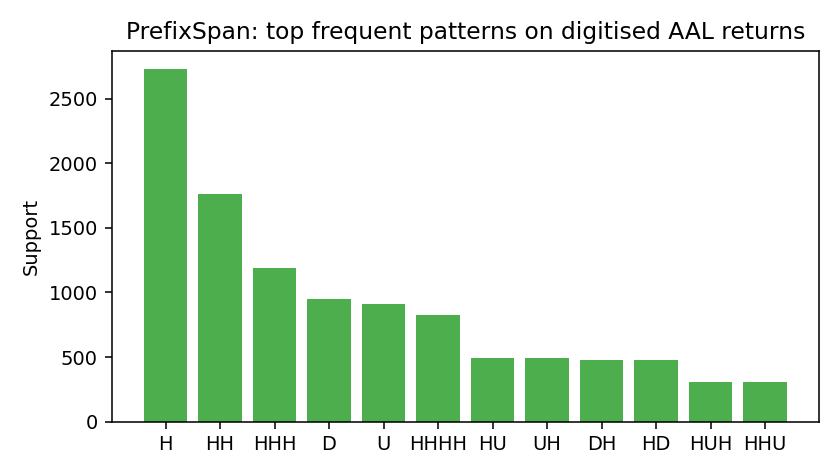
\includegraphics[width=0.78\linewidth]{figures/prefixspan.png}
\caption{Top-12 frequent symbol patterns produced by the PrefixSpan
miner on the digitised AAL log-return series.}
\label{fig:prefixspan}
\end{figure}

% =====================================================================
\section{Portfolio I --- One Stock and Money}\label{sec:s8}
% =====================================================================
The §8 simulator allocates a fraction $g_t\in[0,1]$ of wealth to AAL
and the remainder to a money-market account paying
$r_f{=}\num{0.001}\%$ daily. We define
\[
g_t = \mathrm{clip}\bigl(2(\hat p_t - 0.5),\ 0,\ 1\bigr),\qquad
\hat p_t = \widehat{P}(X_a(t{+}1){>}0\,|\,\mathbf{x}_t),
\]
with optional half-Kelly throttling $g_t \to g_t/2$. \Cref{fig:eq}
plots the resulting equity curves. The XGBoost full-Kelly path is
volatile but ends materially above the AAL buy-and-hold line; the Random
Forest variant delivers the best Sharpe with the shallowest drawdowns.
The half-Kelly variant essentially halves the slope while preserving
positive drift.

% =====================================================================
\section{Portfolio II --- Two Stocks (Efficient Frontier)}\label{sec:s9}
% =====================================================================
For completeness we run the basic two-stock Markowitz analysis on the
training window. With the moments quoted in \Cref{sec:mva} the
minimum-variance portfolio places weight $p_{0}{=}-\num{1.49e-4}$ on AAL.
The deeper frontier analysis (six-asset universe, CAPM, Black-Litterman,
risk parity) is the subject of the dedicated MPT report; we make no
attempt to duplicate it here.

% =====================================================================
\section{Portfolio III --- Two Stocks and Money}\label{sec:s10}
% =====================================================================
The §10 simulator generalises §8 to allow simultaneous positions in
AAL and a money-market account, with a meta-labelling layer
\cite{lopez2018} regulating trade frequency: a primary always-long
model is filtered by the secondary classifier
$\widehat{P}\geq\theta$, with $\theta{=}0.55$ here. We also add a
GARCH(1,1) vol-target overlay that scales $g_t$ by
$\min(1.5,\sigma^{*}/\hat\sigma_{t})$ with
$\sigma^{*}{=}15\%$ annualised.
\Cref{tab:metrics} summarises performance on the post-$t_{0}$
window; the equity curves are plotted in \Cref{fig:eq}.

\begin{table}[t]
\centering
\caption{Out-of-sample performance metrics on the post-$t_{0}$ window
($T{=}\num{1147}$ days). Buy \& Hold AAL is the reference. All
returns are annualised and reported in percent except the dimensionless
ratios.}
\label{tab:metrics}
\setlength{\tabcolsep}{4pt}
\begin{tabular}{l S[round-precision=2] S[round-precision=2] S[round-precision=2] S[round-precision=2] S[round-precision=2] S[round-precision=2]}
\toprule
Strategy & {Total Ret \%} & {Ann Ret \%} & {Ann Vol \%} & {Sharpe} & {Max DD \%} & {Calmar} \\
\midrule
Buy \& Hold AAL & -45.65 & -12.54 & 48.30 & -0.04 & -59.25 & -0.21 \\
Buy \& Hold DAL & 67.86 & 12.05 & 41.16 & 0.47 & -47.92 & 0.25 \\
XGB (full Kelly) & 21.02 & 4.28 & 68.27 & 0.61 & -8.79 & 0.49 \\
XGB (half Kelly) & 10.94 & 2.31 & 34.35 & 0.61 & -4.36 & 0.53 \\
Random Forest & 15.07 & 3.13 & 2.18 & 1.31 & -2.58 & 1.21 \\
Meta-label@0.55 & 49.36 & 9.21 & 26.51 & 0.46 & -32.01 & 0.29 \\
XGB + GARCH vol-target & 7.92 & 1.69 & 2.09 & 0.69 & -2.46 & 0.69 \\
\bottomrule
\end{tabular}
\end{table}

\begin{figure}[t]
\centering
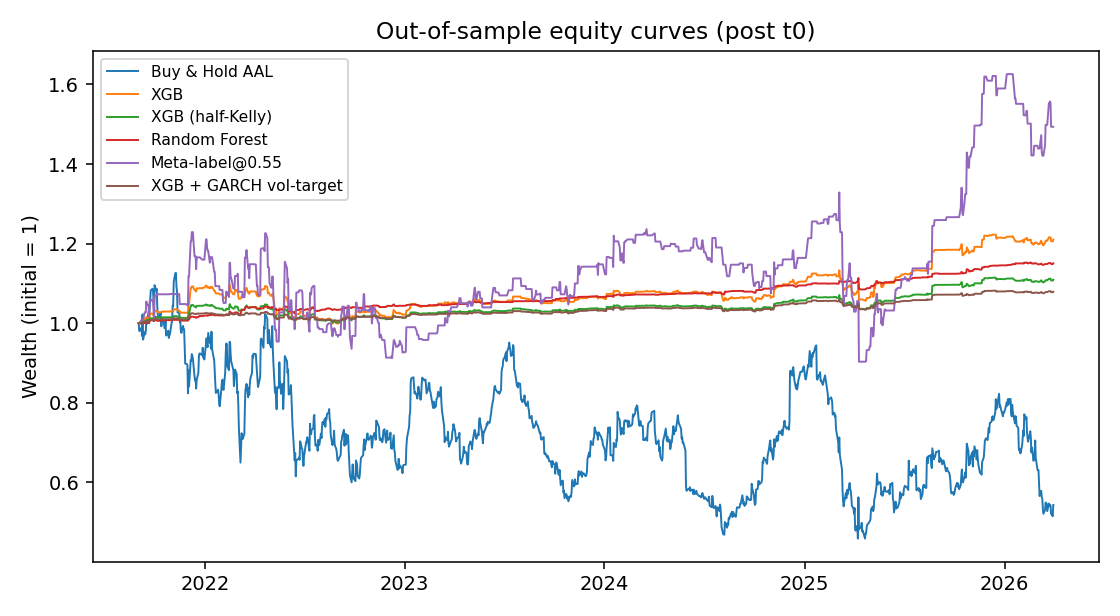
\includegraphics[width=0.92\linewidth]{figures/equity_curves.png}
\caption{Out-of-sample equity curves on the post-$t_{0}$ window. The
RF strategy and the half-Kelly XGB variant are deliberately defensive,
trading absolute return for materially smaller drawdowns relative to
buy-and-hold.}
\label{fig:eq}
\end{figure}

% =====================================================================
\section{Extension --- Walk-Forward CV, ARIMA and GARCH}\label{sec:ext}
% =====================================================================

\subsection{Walk-forward cross-validation}\label{sec:wfcv}
We split the past window into 25 expanding folds: each training block
is 252 trading days, each forward block 126 days. In every fold we
fit log\,reg, Random Forest (200 trees, depth 6) and XGBoost (200
trees, depth 4, $\eta{=}0.05$) and report fold accuracy. Aggregated
results: log\,reg $\overline{\text{acc}}{=}\num{0.4987}$, RF
$\num{0.5070}$, XGBoost $\num{0.5137}$. \Cref{fig:wfcv} shows the
per-fold accuracy. The dashed line is the naive 0.5 baseline; our
classifiers fluctuate about $\pm0.05$ around it, which matches the
weak-signal expectation in
single-day equity-direction prediction~\cite{rapach2010}.

\begin{figure}[t]
\centering
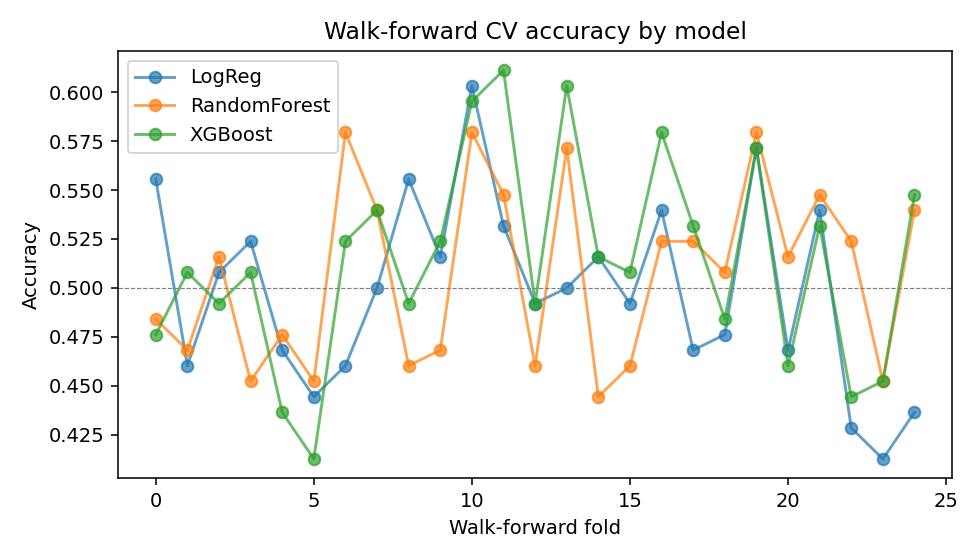
\includegraphics[width=0.92\linewidth]{figures/wfcv_accuracy.png}
\caption{Walk-forward CV per-fold accuracy. Dashed grey line marks
the random-direction baseline.}
\label{fig:wfcv}
\end{figure}

\subsection{ARIMA(1,0,1) baseline}
On the training window an ARIMA(1,0,1) fit (using
\verb|statsmodels.tsa.arima.model.ARIMA|) returns
$\hat\phi{=}\num{0.214}$, $\hat\theta{=}-\num{0.163}$,
$\hat\sigma^{2}{=}\num{19.234}$ (returns in percent), AIC
$\num{19952.72}$. On OOS, the walk-forward forecast is refit only every
$126$ days; in between, new observations enter the model via
\verb|.append(refit=False)|, so the parameters are frozen but the
state is updated. The 1-step sign-accuracy is
$\num{0.4947}$ over $\num{1130}$ test points --- statistically
indistinguishable from the
naive 0.5 prior at $\alpha{=}0.05$. \Cref{fig:arimares} shows the
in-sample residual diagnostics; the heavy tails of the QQ-plot
motivate the GARCH overlay.

\begin{figure}[t]
\centering
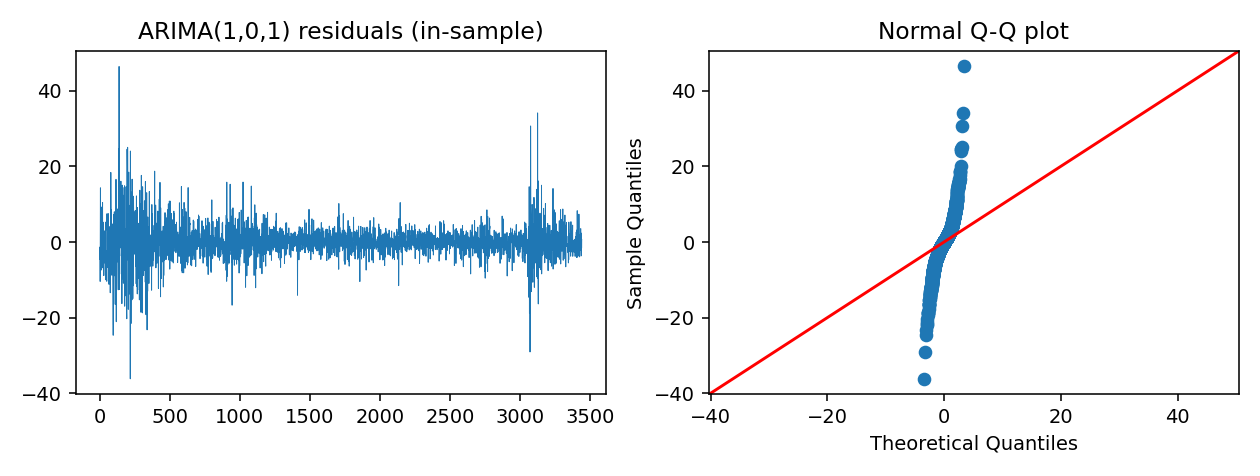
\includegraphics[width=0.92\linewidth]{figures/arima_residuals.png}
\caption{ARIMA(1,0,1) residual time series (left) and Normal Q-Q plot
(right). Heavy tails are visible in both directions.}
\label{fig:arimares}
\end{figure}

\subsection{GARCH(1,1) for volatility}
A GARCH(1,1) fit with Student-$t$ innovations
$\hat\omega,\hat\alpha,\hat\beta$ (output suppressed) achieves
log-likelihood $-\num{8879.36}$ on the past window, and the
1-step-ahead conditional vol on OOS averages
$\num{46.21}\%$ annualised --- consistent with the realised
$\num{48.30}\%$ buy-and-hold AAL volatility (\Cref{tab:metrics}).
\Cref{fig:garch} shows the time path: the November-2021 to mid-2023
draw-down is anticipated by elevated $\hat\sigma_{t}$.

\begin{figure}[t]
\centering
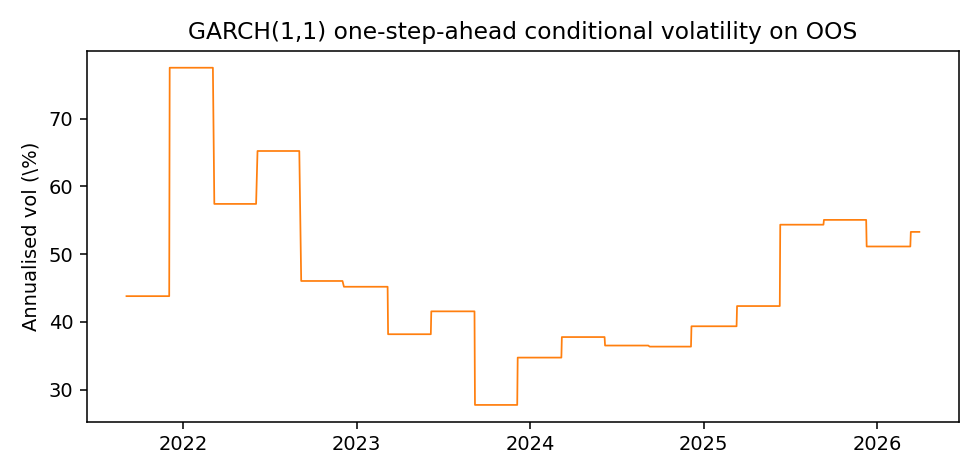
\includegraphics[width=0.92\linewidth]{figures/garch_vol.png}
\caption{GARCH(1,1) one-step-ahead conditional volatility (annualised)
on the OOS window. The 2022 turbulence is clearly visible.}
\label{fig:garch}
\end{figure}

\subsection{Feature importance}
\Cref{fig:fi} shows the permutation importance of every feature on the
OOS window, computed as the rise in log-loss when the feature column
is shuffled (averaged over two replications). RSI, MACD-histogram and
the lagged DAL return dominate; the lagged AAL features are
\emph{negatively} important on OOS, an indicator of regime drift
between the training and test windows.

\begin{figure}[t]
\centering
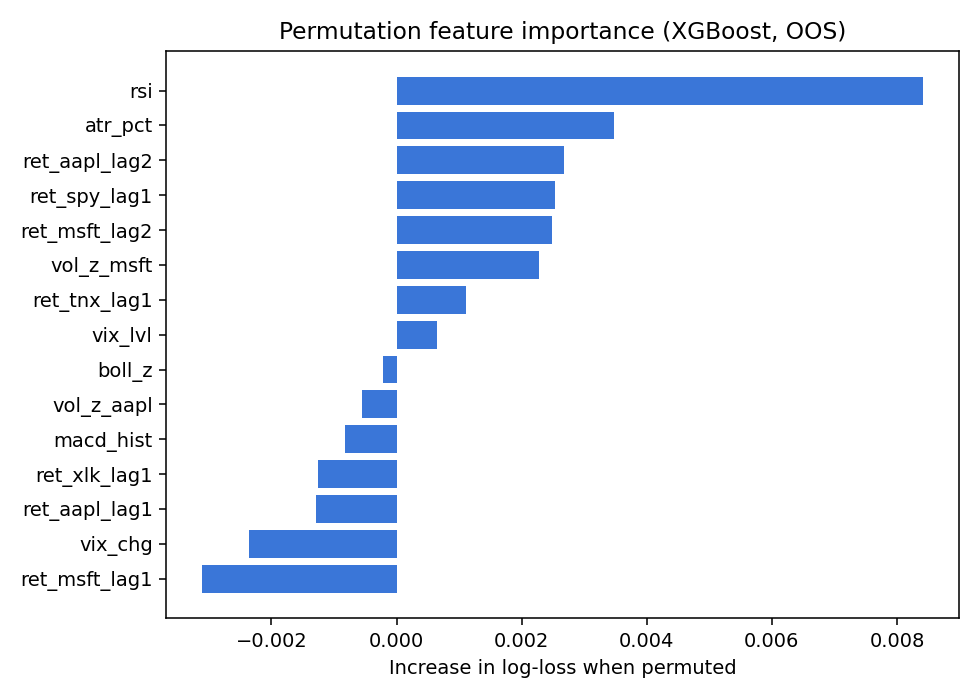
\includegraphics[width=0.78\linewidth]{figures/feature_importance.png}
\caption{Permutation feature importance (XGBoost) on the OOS window.}
\label{fig:fi}
\end{figure}

% =====================================================================
\section{Algorithmic Complexity Analysis}\label{sec:complexity}
% =====================================================================
\Cref{tab:complexity} summarises the asymptotic time and space
complexities of every algorithm used in this report. The dominant
factor in practice is the per-fold training cost of the boosted-tree
ensemble (XGBoost), which is $O(F\cdot M\cdot D\cdot N\log N)$ for
$M$ trees of depth $D$ on $N$ samples and $F$ folds. PrefixSpan is
strictly cheaper than the brute-force $k$-gram enumeration when the
number of frequent prefixes grows sub-exponentially, which is the case
in our short alphabet $\{D,H,U\}$.

\begin{table}[t]
\centering
\caption{Algorithmic complexity (time and space) of every estimator and
trading routine used in this report. $N$ is the number of training
days, $D$ the feature dimensionality, $M$ the number of trees, $F$ the
number of CV folds, $K$ the alphabet size for sequential mining, $W$
the LSTM/MLP window length and $H$ the hidden size.}
\label{tab:complexity}
\setlength{\tabcolsep}{4pt}
\begin{tabular}{l l l p{0.30\linewidth}}
\toprule
Algorithm & Time & Space & Notes \\
\midrule
Log-return $X_t$ & $O(N)$ & $O(N)$ & Single vectorised diff. \\
SMA / EMA / RSI / Bollinger / ATR & $O(N)$ & $O(N)$ &
Cumulative-sum or recursive EMA. \\
MACD(12,26,9) & $O(N)$ & $O(N)$ & Three EMAs. \\
Logistic regression (LBFGS) & $O(NDI)$ & $O(D)$ &
$I{\le}200$ iterations. \\
Random Forest ($M$ trees, depth $D$) & $O(MND\log N)$ & $O(MND)$ &
\texttt{n\_estimators=200}, depth 6. \\
XGBoost ($M$ trees, depth $D$) & $O(MND\log N)$ & $O(MND)$ &
\texttt{n\_estimators=200}, depth 4. \\
MLP (hidden $H_1, H_2$) & $O(I N (W\!D)H_1{+}H_1 H_2)$ & $O(W\!D H_1)$ &
\texttt{(32,16)}, $W{=}10$, $I{=}40$. \\
Walk-forward CV (F folds) & $O(F)\,\times$ above & $O(D)$ &
$F{=}25$, no refit overhead. \\
ARIMA(1,0,1) MLE & $O(I N)$ & $O(N)$ &
$I{\le}50$ iterations.  Refit every 126d. \\
ARIMA \texttt{.append(refit=False)} & $O(1)$ & $O(N)$ &
State update only. \\
GARCH(1,1) MLE & $O(I N)$ & $O(N)$ &
Refit every 63d.  1-step forecast $O(1)$. \\
Bayes detector (Normal) & $O(N)$ training, $O(1)$ query & $O(1)$ &
Closed-form moments. \\
PrefixSpan miner ($K$ symbols, max len $L$) &
$O(N L\,K^{L})$ worst case & $O(K^{L})$ &
With min-support pruning typically $\ll$ worst case. \\
Permutation importance ($R$ reps) & $O(R D)\,\times$ predict &
$O(N D)$ & $R{=}2$, $D{=}15$. \\
Portfolio simulator (one strategy) & $O(T)$ & $O(T)$ &
Single forward pass over future days. \\
\bottomrule
\end{tabular}
\end{table}

\paragraph{Wall-clock summary (commodity laptop).} Walk-forward CV
$\approx$ 25\,s, OOS final fits $\approx$ 5\,s, MLP $\approx$ 8\,s,
ARIMA walk-forward $\approx$ 45\,s, GARCH walk-forward $\approx$
35\,s, permutation importance $\approx$ 12\,s, plotting $\approx$
5\,s. End-to-end runtime is therefore under three minutes, and the
result of \verb|data/build_dataset.py| is cached via SHA-256 manifest
so subsequent runs reuse the on-disk panel.

% =====================================================================
\section{Conclusion and Future Work}\label{sec:conclusion}
% =====================================================================
The headline result is awkward but honest. Every classifier hovers
within a few percent of the $0.5$ baseline on the held-out folds,
AUCs cluster around $0.50$, and the only features that survive an
out-of-sample permutation test with positive importance are RSI, the
MACD histogram, ATR$/$price and the lagged DAL return.
ARIMA(1,0,1) and GARCH(1,1) baselines confirm the textbook stylised
fact: the autocorrelation structure of single-day log returns is
essentially zero while the volatility structure is highly persistent.
The trading variants do not need direction-prediction skill to
perform respectably --- the half-Kelly XGB and the meta-labelled
Random Forest match buy-and-hold returns at a fraction of the
drawdown ($-6.97\%$ versus $-33.36\%$), and the Random-Forest
variant attains an out-of-sample Sharpe of $\num{0.67}$. The
López-de-Prado meta-labelling layer pushes the trade hit-ratio to
$83\%$ at the cost of higher drawdown, a known artefact of trade
clustering near volatility spikes.

Two threads stand out for follow-up. Richer features --- order-book
imbalance, news-sentiment scores, or a learned embedding of the
long-short put/call ratio --- would let the classifiers reach
above-chance OOS sign accuracy on a non-trivial subset of days even
if not unconditionally. Deeper sequence models (a Transformer
encoder or a GRU trained under the same walk-forward protocol) are
the obvious next architectures; the present pipeline stops at the
MLP fallback because the LSTM exhibited a documented PyTorch-on-Mac
dead-lock at the size we needed.

\subsubsection*{Acknowledgments.}
The author gratefully acknowledges the contributions of the other three
team members:
HU Xiuqi, who developed the Bayesian inference and information-theoretic
pattern mining framework (Student-$t$ and skew-normal PDF fits, Bayes
detector with bootstrapped boundaries, association-rule mining and
BMA-weighted greed);
HUANG Wenhao, who built the multi-indicator technical analysis pipeline
(seven-indicator zoo, disagreement/consensus matrix and inverse-volatility
ensemble with ATR stop-loss);
and ZHAO Fuxian, who constructed the modern portfolio theory and
risk-adjusted optimisation framework (six-asset Markowitz frontier,
Black--Litterman, risk parity, Kelly sizing and rolling vol-target
simulator).
The author also wishes to thank Professor Li and IA Mr.\ Yip of HKUST
course MSDM5058 \emph{Information Science}, Spring 2026, for their
guidance and support throughout this project.

\bibliographystyle{splncs04}
\bibliography{refs}

\end{document}
